\documentclass[addpoints]{exam}
\usepackage{amsmath,amsthm,amssymb,url}
\usepackage{cancel}
\usepackage{algorithm}
\usepackage{algorithmic}
\usepackage{graphicx}
\usepackage{float}
\usepackage{upgreek}
\usepackage{bm}
\usepackage{units}
\usepackage[pdftex]{hyperref}
\usepackage{tikz}
\usepackage{subcaption}
\usetikzlibrary{shapes,snakes}

\def\checkmark{\hspace{.5em}\tikz\fill[scale=0.4](0,.35) -- (.25,0) -- (1,.7) -- (.25,.15) -- cycle;} 
\DeclareMathOperator*{\pprime}{\prime \prime}
\renewcommand{\algorithmicrequire}{\textbf{Input:}}
\renewcommand{\algorithmicensure}{\textbf{Output:}}
\newcommand{\BigO}[1]{\mathcal{O}\left( #1\right)}
\newcommand{\D}[1]{\left. #1 \right|_{i}^{n}}
\newcommand{\C}[1]{\cancel{ #1}}
\newcommand{\DC}[1]{\C{\D{ #1}}}
\newcommand{\Dx}{\Delta x}
\newcommand{\Dy}{\Delta y}
\newcommand{\Dt}{\Delta t}
\newcommand{\Dtp}{\Delta t^{\prime}}


\newtheorem{lemma}{Lemma}[section]
\newcommand{\var}{\text{Var}}
\title{ME EN 6720: Homework 3}
\date{Due Date: March 21, 2016}
\author{Christopher Mertin}
\begin{document}
\maketitle
%\begin{center}
%\fbox{\fbox{\parbox{5.5in}{\centering
%This assignment has \numquestions\ questions, for a total of \numpoints\
%points.
%Unless otherwise specified, complete and reasoned arguments will be
%expected for all answers. 
%}}}
%\end{center}

\qformat{Question \thequestion: \thequestiontitle\dotfill}
\pointname{}
\bonuspointname{}
\pointformat{[\bfseries\thepoints]}

\printanswers



\begin{questions}
\titledquestion{Numerical Methods and the Vorticity-Streamfunction}
Consider the flow in a lid driven cavity illustrated in the figure below. The cavity is square and flow in the cavity is driven by an upper plate moving at a constant velosity of $U$. The Reynolds number for the flow is $R_{e} = Uw/\nu = 100$. Solve for the steady state flow in the cavity using the vorticity-streamfunction method outlined in Lecture 12 (also see Ferziger pg. 181 and Tannehill {\em et. al}, pg. 650). Construct a second order finite difference solution for the problem (for both $\omega$ and $\Psi$) and solve it using the following schemes:
\begin{enumerate}
\item Jacobi Iterations
\item Gauss-Seidel
\item Gauss-Seidel with Successive Over-Relaxations ({\sc Sor})
\item Gauss-Seidel with a 1-level nested Multigrid Method
\end{enumerate}

For {\bf extra credit}, use a solver package for the following:
\begin{enumerate}
\setcounter{enumi}{4}
\item Preconditioned Conjugate Gradient Method ({\sc Pcg})
\item Generalized Minimal Residual Method ({\sc Gmres})
\end{enumerate}

Use a uniform mesh to solve your problem with $N_{x}=N_{y}=50$ points in the horizontal $x$ and vertical $y$ directions respectively. Start the iterations with $u(x,y)=v(x,y)=0$ (you can also explore using $u(x,y)=U$ and $v(x,y)=0$). For a fixed convergence criteria (on the finite grid for multigrid methods), which scheme converges fastest? How do all the schemes compare to each other (measured by performance)? What is the optimum value of the relaxation coefficient for the {\sc Sor} scheme? Present your results by plotting the streamlines for each scheme overlaid on a filled contour (or pseudo color) plot of the vorticity in the cavity. Also include a table comparing the number of iterations and total execution times for each method along with a short discussion. If you do the extra credit, with the {\sc Pcg} and {\sc Gmres} methods, report at least the minimum total time.

\begin{figure}[H]
\centering
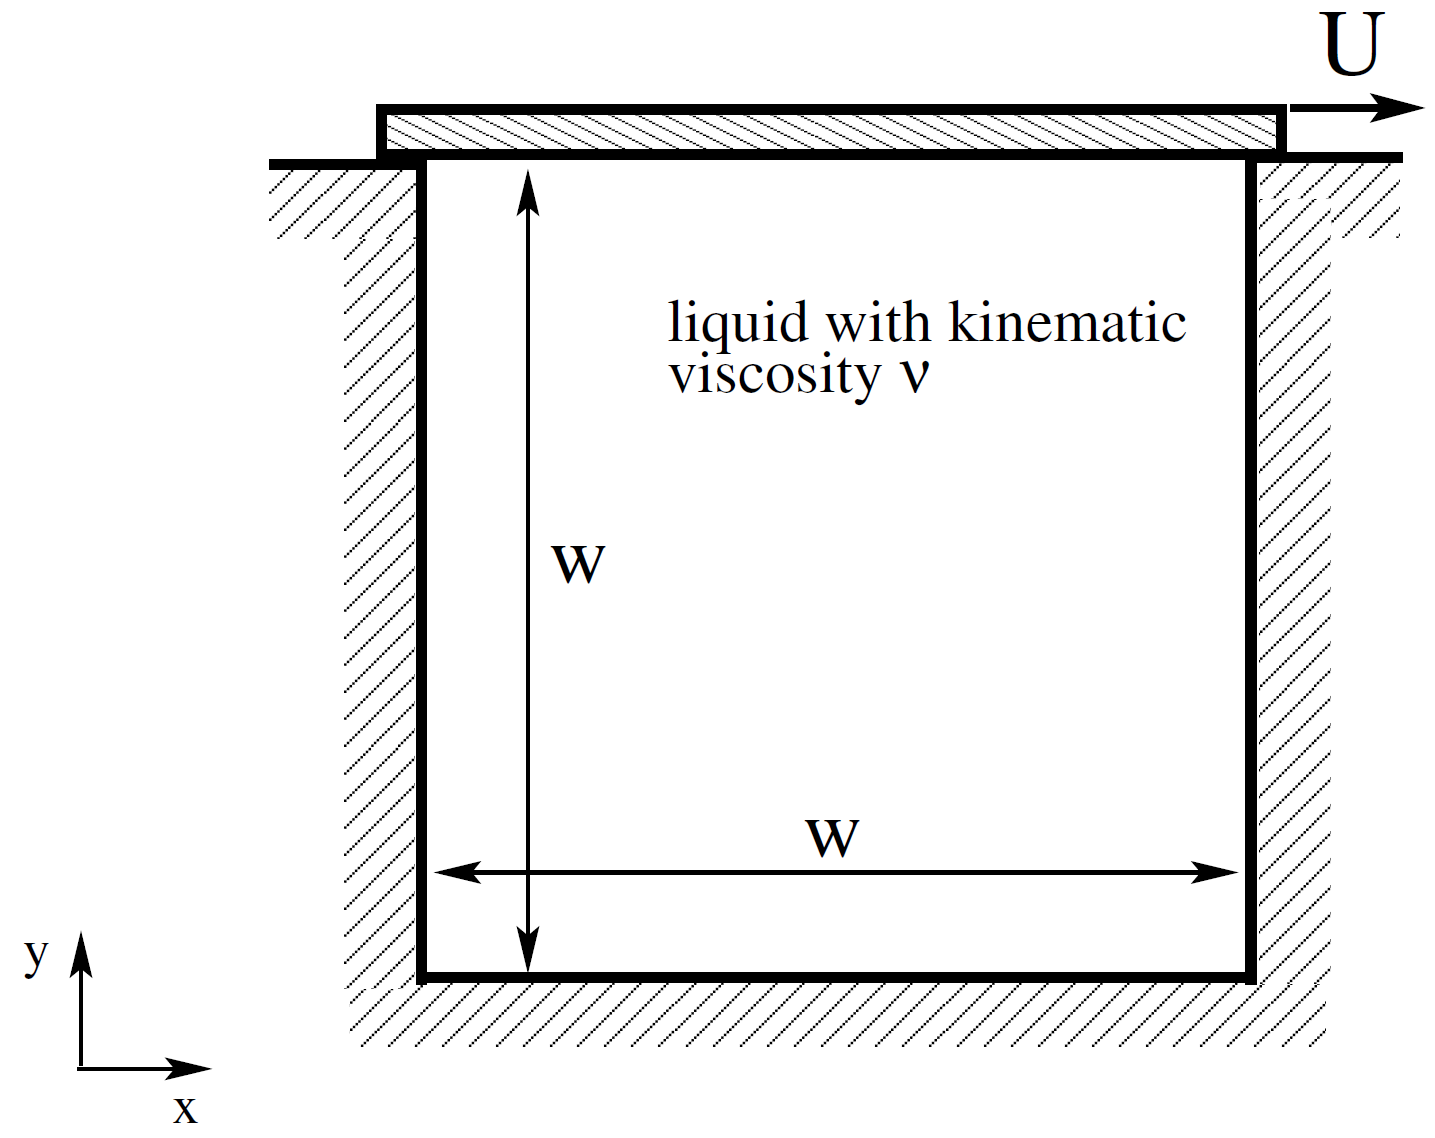
\includegraphics[width=.4\textwidth]{fig1.png}
\caption{Given Problem}
\end{figure}

\begin{solution}
The 2D vorticity $(\omega)$ is represented as

\begin{align}
\omega &= \boldsymbol{\nabla}\times \mathbf{V}\\
\intertext{with the scalar value being}
\omega &= \frac{\partial v}{\partial x} - \frac{\partial u}{\partial y}\\
\intertext{and the relation to the velocity from the streamfunction $\psi$ is}
\frac{\partial \psi}{\partial y} &= u\label{eq:psiu}\\
\frac{\partial \psi}{\partial x} &= -v\label{eq:psiv}\\
\intertext{However, we also need a {\em time-evolution} scheme for how the system evolves. This is done with the {\em vorticity transport equation}, which is represented as}
\frac{D\omega}{Dt} &= \cancel{\frac{\partial \omega}{\partial t}} + (\vec{u}\cdot \boldsymbol{\nabla})\vec{\omega} = \nu\nabla^{2}\omega
\intertext{where the first term cancels in the case of incompressibility, leaving the 2D case as being}
\frac{D\omega}{Dt} &= u\frac{\partial \omega}{\partial x} + v\frac{\partial \omega}{\partial y} = \nu\left[\frac{\partial^{2}\omega}{\partial x^{2}} + \frac{\partial^{2}\omega}{\partial y^{2}}\right]\\
\intertext{which from Equation (\ref{eq:psiu}) and Equation (\ref{eq:psiv}) we get}
\frac{D\omega}{Dt} &= \frac{\partial \psi}{\partial y}\frac{\partial \omega}{\partial x} - \frac{\partial \psi}{\partial x}\frac{\partial \omega}{\partial y} = \nu\left[\frac{\partial^{2}\omega}{\partial x^{2}} + \frac{\partial^{2}\omega}{\partial y^{2}}\right]\label{eq:advec}\\
\intertext{We can also relate the streamfunction and the vorticity as being the Poisson equation of}
\nabla^{2}\psi &= -\omega\label{eq:poisson}
\end{align}

Using these above relations, we can solve the Navier-Stokes Equations in streamfunction and vorticity form in the following steps:

\begin{enumerate}
\item Specify initial values for $\omega$ and $\psi$ at $t=0$
\item Solve the vorticity transport equation for $\omega$ at each interior point for $t + \Delta t$
\item Iterate for new values of $\psi$ at all points by solving the Poisson Equation using the new values of $\omega$
\item Find the velocity components from $u = \psi_{y}$ and $v = -\psi_{x}$
\item Determine the values of $\omega$ on the boundaries using $\psi$ and $\omega$ values at the interior points
\item Return to step 2 if not converged
\end{enumerate}

Before doing so though, we need to define the boundary conditions of the system. These can be seen in Figure~\ref{fig:boxbc}.

\begin{figure}[H]
\centering
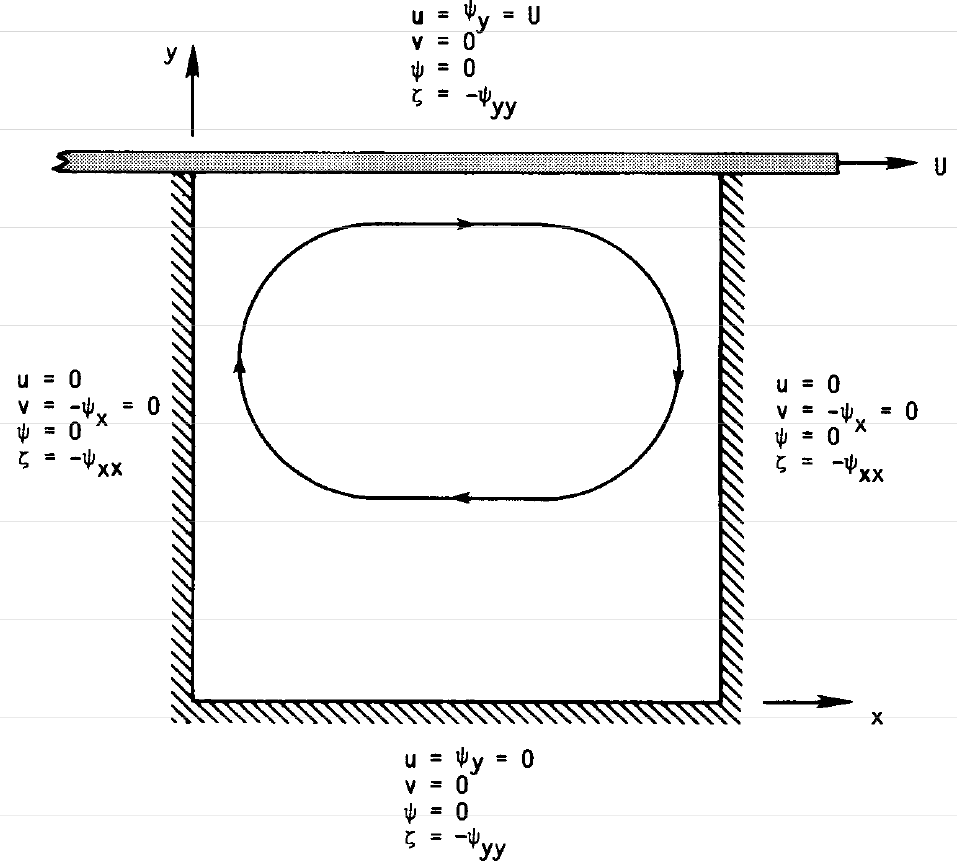
\includegraphics[width=.5\textwidth]{box_bc.png}
\caption{Driven Cavity Problem with Boundary Conditions, extracted from \cite{box}}
\label{fig:boxbc}
\end{figure}

Finally, we need to discretize the above equations so that we can solve them numerically. When discritizing, we get the {\em vorticity transport equation} as being

\begin{align}
\omega_{i,j}^{n+1} &= \omega_{i,j}^{n} + \Delta t \left[ \left(\frac{\psi_{i,j+1}-\psi_{i,j-1}}{\Delta}\right)\left(\frac{\omega_{i+1,j}-\omega_{i-1,j}}{\Delta}\right) - \left(\frac{\psi_{i+1,j}-\psi_{i-1,j}}{\Delta}\right)\left(\frac{\omega_{i,j+1}-\omega_{i,j-1}}{\Delta}\right)\right.\nonumber\\
&\phantom{aaaaaaaaaaa}\left.+ \nu\left(\frac{\omega_{i+1,j}+\omega_{i-1,j}+\omega_{i,j+1}+\omega_{i,j-1}-4\omega_{i,j}}{\Delta^{2}}\right)\right]
\intertext{where $\Delta$ represents $\Delta x$ and $\Delta y$ since it's a uniform grid. The vorticity at the walls are}
\omega_{N,j} &= \frac{2\left(\psi_{i,j-1} - \psi_{i,j}\right)}{\Delta^{2}} + U\frac{2}{\Delta}\\
\omega_{1,j} &= \frac{2\left(\psi_{i,j} - \psi_{i,j+1}\right)}{\Delta^{2}} + 0\\
\omega_{i,1} &= \frac{2\left(\psi_{i,j} - \psi_{i+1,j}\right)}{\Delta^{2}} + 0\\
\omega_{i,N} &= \frac{2\left(\psi_{i-1,j} - \psi_{i,j}\right)}{\Delta^{2}} + 0
\intertext{which comes about because we set $\psi = 0$ along the boundaries, so the $\psi_{i,j}$ terms cancel, and the second term is $\frac{\partial \psi_{i,j}}{\partial y}$ or $\frac{\partial \psi_{i,j}}{\partial x}$ depending on the boundary, which is zero for every boundary {\em except} the top. Finally, we can solve the Poisson Equation, Equation (\ref{eq:poisson}) in the following two ways, by Matrix and Matrix-free methods. For the Matrix, since we want the {\em boundary} values of $\psi$ to be zero, on a $6\times 6$ grid, the matrix would be of the form}
\mathbf{A} &= \left[ \begin{array}{c c c c c c c c c c c c c c c c }
 4 & -1 &  0 &  0 & -1 &  0 &  0 &  0 &  0 &  0 &  0 &  0 &  0 &  0 &  0 &  0\\
-1 &  4 & -1 &  0 &  0 & -1 &  0 &  0 &  0 &  0 &  0 &  0 &  0 &  0 &  0 &  0\\
 0 & -1 &  4 & -1 &  0 &  0 & -1 &  0 &  0 &  0 &  0 &  0 &  0 &  0 &  0 &  0\\
 0 &  0 & -1 &  4 &  0 &  0 &  0 & -1 &  0 &  0 &  0 &  0 &  0 &  0 &  0 &  0\\
-1 &  0 &  0 &  0 &  4 & -1 &  0 &  0 & -1 &  0 &  0 &  0 &  0 &  0 &  0 &  0\\
 0 & -1 &  0 &  0 & -1 &  4 & -1 &  0 &  0 & -1 &  0 &  0 &  0 &  0 &  0 &  0\\
 0 &  0 & -1 &  0 &  0 & -1 &  4 & -1 &  0 &  0 & -1 &  0 &  0 &  0 &  0 &  0\\
 0 &  0 &  0 & -1 &  0 &  0 & -1 &  4 &  0 &  0 &  0 & -1 &  0 &  0 &  0 &  0\\
 0 &  0 &  0 &  0 & -1 &  0 &  0 &  0 &  4 & -1 &  0 &  0 & -1 &  0 &  0 &  0\\
 0 &  0 &  0 &  0 &  0 & -1 &  0 &  0 & -1 &  4 & -1 &  0 &  0 & -1 &  0 &  0\\
 0 &  0 &  0 &  0 &  0 &  0 & -1 &  0 &  0 & -1 &  4 & -1 &  0 &  0 & -1 &  0\\
 0 &  0 &  0 &  0 &  0 &  0 &  0 & -1 &  0 &  0 & -1 &  4 &  0 &  0 &  0 & -1\\
 0 &  0 &  0 &  0 &  0 &  0 &  0 &  0 & -1 &  0 &  0 &  0 &  4 & -1 &  0 &  0\\
 0 &  0 &  0 &  0 &  0 &  0 &  0 &  0 &  0 & -1 &  0 &  0 & -1 &  4 & -1 &  0\\
 0 &  0 &  0 &  0 &  0 &  0 &  0 &  0 &  0 &  0 & -1 &  0 &  0 & -1 &  4 & -1\\
 0 &  0 &  0 &  0 &  0 &  0 &  0 &  0 &  0 &  0 &  0 & -1 &  0 &  0 & -1 &  4
\end{array}\right]\label{eq:mat}
\intertext{where every $N-1$ rows have a zero in the upper diagonal element, and every $N$ rows have a zero in the lower diagonal part. These zeros are used to {\em force} the boundary conditions of having a zero element. As can be seen, the majority of the terms are zero, so to speed up computations, only the non-zero diagonals can be stored and the matrix manipulations can be specified to this matrix structure to both reduce storage and computational cost. Alternatively, by discritizing Equation~(\ref{eq:poisson}), we can use the Matrix-free method which produces the equation}
\psi_{i,j} &= \psi_{i+1,j} + \psi_{i-1,j} + \psi_{i,j+1} + \psi_{i,j-1} + \Delta^{2}\omega_{i,j}\label{eq:matfree}
\end{align}
where with Equation~(\ref{eq:mat}) or Equation~(\ref{eq:matfree}) we can use any iterative method to solve the system. The Pseudocode for the most popular methods are defined below

\begin{algorithm}[H]
\caption{Jacobi Iterative}
\begin{algorithmic}
\REQUIRE{$\mathbf{A}\in \mathbb{R}^{N\times N}$, $\vec{x}^{(0)}\in \mathbb{R}^{N\times 1}$, $\vec{b}\in \mathbb{R}^{N\times 1}$, $tol$erance, $MAX$ iterations}
\ENSURE{$\vec{x}^{(k)} = \mathbf{A}^{-1}\vec{b}$}
\FOR{$k = 1$ \TO $MAX$}
    \FOR{$i = 1$ \TO $N$}
        \STATE{$x_{i}^{(k)} = \frac{-\sum_{j=1,j\neq i}^{N}\left(a_{i,j}x_{j}^{(k-1)}\right) + b_{i}}{a_{i,i}}$}
    \ENDFOR
    \IF{$\left|\left|x^{(k)}-x^{(k-1)}\right|\right|<tol$}
       \RETURN{$x^{(k)}$}
    \ENDIF
\ENDFOR
\end{algorithmic}
\label{alg:jacobi}
\end{algorithm}

\begin{algorithm}[H]
\caption{Gauss-Seidel}
\begin{algorithmic}
\REQUIRE{$\mathbf{A}\in \mathbb{R}^{N\times N}$, $\vec{x}^{(0)}\in \mathbb{R}^{N\times 1}$, $\vec{b}\in \mathbb{R}^{N\times 1}$, $tol$erance, $MAX$ iterations}
\ENSURE{$\vec{x}^{(k)} = \mathbf{A}^{-1}\vec{b}$}
\FOR{$k = 1$ \TO $MAX$}
    \FOR{$i = 1$ \TO $N$}
        \STATE{$x_{i}^{(k)} = \frac{-\sum_{j=1}^{i-1}\left(a_{i,j}x_{j}^{(k)}\right)-\sum_{j=i+1}^{N}\left(a_{i,j}x_{j}^{(k-1)}\right) + b_{i}}{a_{i,i}}$}
    \ENDFOR
    \IF{$\left|\left|x^{(k)}-x^{(k-1)}\right|\right|<tol$}
       \RETURN{$x^{(k)}$}
    \ENDIF
\ENDFOR
\end{algorithmic}
\end{algorithm}

\begin{algorithm}[H]
\caption{Gauss-Seidel ({\sc Sor})}
\begin{algorithmic}
\REQUIRE{$\mathbf{A}\in \mathbb{R}^{N\times N}$, $\vec{x}^{(0)}\in \mathbb{R}^{N\times 1}$, $\vec{b}\in \mathbb{R}^{N\times 1}$, $\zeta$ {\sc Sor} parameter, $tol$erance, $MAX$ iterations}
\ENSURE{$\vec{x}^{(k)} = \mathbf{A}^{-1}\vec{b}$}
\FOR{$k = 1$ \TO $MAX$}
    \FOR{$i = 1$ \TO $N$}
        \STATE{$x_{i}^{(k)} = (1-\zeta)x_{i} + \frac{\zeta\left(-\sum_{j=1}^{i-1}\left(a_{i,j}x_{j}^{(k)}\right)-\sum_{j=i+1}^{N}\left(a_{i,j}x_{j}^{(k-1)}\right) + b_{i}\right)}{a_{i,i}}$}
    \ENDFOR
    \IF{$\left|\left|x^{(k)}-x^{(k-1)}\right|\right|<tol$}
       \RETURN{$x^{(k)}$}
    \ENDIF
\ENDFOR
\end{algorithmic}
\label{alg:sor}
\end{algorithm}

\begin{algorithm}[H]
\caption{MultiGrid \cite{multigrid}}
\begin{algorithmic}
\REQUIRE{$\mathbf{A}\in \mathbb{R}^{N\times N}$, $\vec{x}\in \mathbb{R}^{N\times 1}$, $\vec{b}\in \mathbb{R}^{N\times 1}$, $\ell$ level, $\nu_{1}$, $\nu_{2}$}
\ENSURE{$\vec{x}^{(k)} = \mathbf{A}^{-1}\vec{b}$}
\IF{$\ell = 0$}
   \STATE{Solve $\mathbf{A}\vec{x} = \vec{b}$ Iteratively}
   \COMMENT{Gauss-Seidel}
\ELSE
    \STATE{$x_{\ell} = S_{\ell}^{\nu_{1}}\left(x_{\ell},b_{\ell}\right)$}
    \STATE{$d_{\ell-1} = R_{\ell - 1,\ell}\left(b_{\ell}-A_{\ell}x_{\ell}\right)$}
    \STATE{$v_{\ell-1} = \vec{0}$}
    \FOR{$i = 0$ \TO $\gamma$}
        \STATE{MultiGrid$(v_{\ell-1},d_{\ell-1},\ell-1)$}
        \COMMENT{Recursive}
    \ENDFOR
    \STATE{$x_{\ell} = x_{\ell} + P_{\ell,\ell-1}v_{\ell-1}$}
    \STATE{$x_{\ell} = S_{\ell}^{\nu_{2}}\left(x_{\ell},b_{\ell}\right)$}
\ENDIF
\end{algorithmic}
\end{algorithm}

\begin{algorithm}[H]
\caption{Pre-Conjugate Gradient \cite{pcg}}
\begin{algorithmic}
\REQUIRE{$\mathbf{A}\in \mathbb{R}^{N\times N}$, $\vec{x}^{(0)}\in \mathbb{R}^{N\times 1}$, $\vec{b}\in \mathbb{R}^{N\times 1}$, $\mathbf{M}$ preconditioner, $MAX$ iterations, $tol$erance}
\ENSURE{$\vec{x} = \mathbf{A}^{-1}\vec{b}$}
\STATE{$i\leftarrow 0$}
\STATE{$r\leftarrow \vec{b} - \mathbf{A}\vec{x}$}
\STATE{$d\leftarrow \mathbf{M}^{-1}r$}
\COMMENT{Common choice of $\mathbf{M} = \text{Diag}(\mathbf{A})$}
\STATE{$\delta_{new}\leftarrow r^{T}d$}
\STATE{$\delta_{0}\leftarrow \delta_{new}$}
\WHILE{$i<MAX$ \AND $\delta_{new}>tol^{2}\delta_{0}$}
      \STATE{$q\leftarrow \mathbf{A}d$}
      \STATE{$\alpha \leftarrow \frac{\delta_{new}}{d^{T}q}$}
      \STATE{$x \leftarrow x + \alpha d$}
      \IF{$i$ is divisible by 50}
         \STATE{$r \leftarrow b - \mathbf{A}x$}
      \ELSE
         \STATE{$r \leftarrow r - \alpha q$}
      \ENDIF
      \STATE{$s \leftarrow \mathbf{M}^{-1}r$}
      \STATE{$\delta_{old} \leftarrow \delta_{new}$}
      \STATE{$\delta_{new} \leftarrow r^{T}s$}
      \STATE{$\beta \leftarrow \frac{\delta_{new}}{\delta_{old}}$}
      \STATE{$d \leftarrow s + \beta d$}
      \STATE{$i \leftarrow i + 1$}
\ENDWHILE
\end{algorithmic}
\end{algorithm}

\begin{algorithm}[H]
\caption{{\sc Gmres} \cite{gmres}}
\begin{algorithmic}
\REQUIRE{$\mathbf{A}\in \mathbb{R}^{N\times N}$, $\vec{x}^{(0)}\in \mathbb{R}^{N\times 1}$, $\vec{b}\in \mathbb{R}^{N\times 1}$}
\ENSURE{$\vec{x} = \mathbf{A}^{-1}\vec{b}$}
\STATE{$r_{0} = b - \mathbf{A}x_{0}$}
\STATE{$\beta = \left|\left| r_{0}\right|\right|_{2}$}
\STATE{$v_{1} = r_{0}/\beta$}
\STATE{Define the $\mathbb{R}^{(m+1)\times m}$ matrix $H_{m}$ and set elements $h_{i,j}$ to zero}
\FOR{$j = 1$ \TO $m$}
    \STATE{Compute $w_{j} = Av_{j}$}
    \FOR{$i = 1$ \TO $j$}
        \STATE{$h_{i,j} = (w_{j},v_{i})$}
        \STATE{$w_{j} = w_{j} - h_{i,j}v_{i}$}
    \ENDFOR
    \STATE{$h_{j+1,j} = \left|\left| w_{j}\right|\right|_{2}$}
    \IF{$h_{j+1,j} = 0$}
       \STATE{Compute $y_{j}$ as the Minimizer of $\left|\left|\beta e_{1} - H_{j}y\right|\right|_{2}^{2}$}
       \RETURN{$x_{j} = x_{0} + V_{j}y_{j}$}
    \ENDIF
    $v_{j+1} = w_{j}/h_{j+1,j}$
\ENDFOR
       \STATE{Compute $y_{m}$ as the Minimizer of $\left|\left|\beta e_{1} - H_{m}y\right|\right|_{2}^{2}$}
       \RETURN{$x_{m} = x_{0} + V_{m}y_{m}$}
\end{algorithmic}
\end{algorithm}

All of these above algorithms can be found in {\tt Matrix.h} which implements them for the given pentagonal matrix that is defined above.

Unfortunately, I was unable to obtain the correct solution for the numerical results, which limits the amount that I can respond to this question. Using {\em any} of the above numerical methods produced a solution as portrayed in Figure~\ref{fig:vorticity}

\begin{figure}[H]
\centering
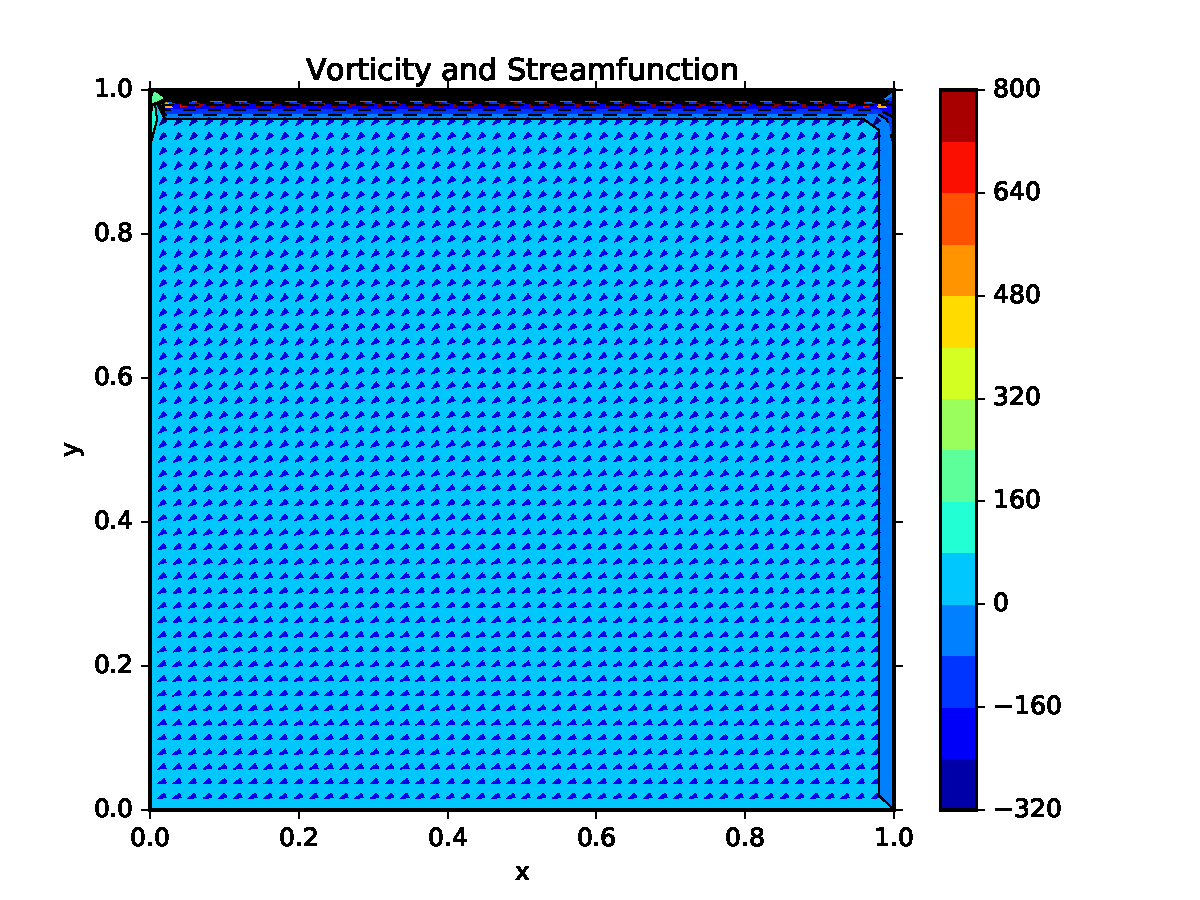
\includegraphics[width = .8\textwidth]{plot_vorticity.pdf}
\caption{``Typical'' results from the solver}
\label{fig:vorticity}
\end{figure}

I was unable to obtain results as it seems the boundary conditions are not ``sticking'' for some reason. Therefore, I was not able to test the iterative solvers on how quick they can solve the system. However, in lieu of this, I decided to test the number of iterations that each iterative solver took on an {\em arbitrary} system so that some results could be reported.

From Algorithm~\ref{alg:sor}, there is an optimal parameter $\zeta$ which needs ot be determined to find out the most {\em efficient} choice. The table of the values of $\zeta$ with the number of iterations can be found in Table~\ref{table:sor}

\begin{table}[H]
\centering
\begin{tabular}{l r}
\hline\hline
$\zeta$ & Iterations\\
\hline
0.1 & 26\\
0.2 & 20\\
0.3 & 15\\
0.4 & 11\\
0.5 & 10\\
0.6 & 8\\
0.7 & 7\\
0.8 & 7\\
0.9 & 6\\
1.0 & 6\\
\hline\hline
\end{tabular}
\caption{Values of $\zeta$ for {\sc Sor}}
\label{table:sor}
\end{table}

Note, when $\zeta = 1.0$, it is reduced down to the normal Gauss-Seidel method. From this table, the optimal value of $\zeta$ can be chosen. From here, the overall number of iterations from {\em all} the methods could be determined and can be seen in Table~\ref{table:iterative}

\begin{table}[H]
\centering
\begin{tabular}{l r}
\hline\hline
Iterative Scheme & Iterations\\
\hline
Jacobi & 11\\
Gauss-Seidel & 6\\
{\sc Sor} & 6\\
{\sc Pcg} & 114\\
\hline\hline
\end{tabular}
\caption{Iterations of Iterative Methods}
\label{table:iterative}
\end{table}

For the above iterations, $\zeta = 0.9$ was chosen for the experiments. The preconditioner for {\sc Pcg} was chosen to be $\text{Diag}(\mathbf{A})$ for the system. Changing this could vary the number of iterations in the solver greatly, though this was chosen as the ``default'' for the implementation.
\end{solution}


\end{questions}

\begin{thebibliography}{99}
\bibitem{box}John C. Tannehill, {\em et. al}, {\em Computational Fluid Mechanics and Heat Transfer}
\bibitem{multigrid}Christian Wagner, {\em Introduction to Algebraic Multigrid}, \url{http://perso.uclouvain.be/alphonse.magnus/num2/amg.pdf}
\bibitem{pcg}Jonathan Richard Shewchuck, {\em An Introduction to the Conjugate Gradient Method Without the Agonizing Pain}, \url{https://www.cs.cmu.edu/~quake-papers/painless-conjugate-gradient.pdf}
\bibitem{gmres}Jens Markus Melenk, \url{www.asc.tuwien.ac.at/~melenk/teach/iterative_SS07/part5.ps}
\end{thebibliography}

\end{document}

%%% Local Variables:
%%% mode: latex
%%% TeX-master: t
%%% End:
